\documentclass[12pt,a4paper]{report}
\usepackage[latin1]{inputenc}
\usepackage{amsmath}
\usepackage{amsfonts}
\usepackage{amssymb}
\usepackage{graphicx}
\usepackage{listings}
\usepackage{color}
\usepackage{hyperref}
\usepackage{framed}
\hypersetup{colorlinks=true, linkcolor=blue}
\usepackage[hypcap]{caption}
\graphicspath{ {./Docimages/} }
\setcounter{secnumdepth}{3}
\setcounter{tocdepth}{3}

\usepackage{mathtools}
\DeclarePairedDelimiter\abs{\lvert}{\rvert}
\begin{document}
\lstset{language=Java} 
\title{Android application for\\resistor value detection}
\author{Opra Istv�n Bal�zs\and Mich\`ele Gouiffes\\consultant}
\maketitle
\tableofcontents
\chapter{Introduction}
\section{Overview}
This report is intended to serve two purposes: firstly to give a brief overview of the work process I followed during my internship at Universit� Paris-Sud during the summer of 2013; moreover to give a more detailed description of the artifacts created during said internship -- namely the Android application package and the Matlab program.

The latter part can also be used as a guide on how to continue work on the project.
\section{About the topic}
My consultant, Mich\`ele Gouiffes suggested two possible \mbox{image-processing} topics for me at the beginning of my internship.

One was related to tracking algorithms: PhD students developed video tracking solutions using mean-shift and covariance tracking, and my task would have been to improve these by the introduction of Kalman-filtering.

The other \mbox{task -- which} I ended up \mbox{choosing -- was} the creation of an Android-based smartphone\slash tablet application which would replace an Ohm meter for through hole mounted resistors. It would achieve this by using the camera to detect the color code on such resistors.

This second topic was suggested by a laboratory course instructor of Paris-Sud, who thought that such an application would be very helpful for students in the laboratory course, as they wouldn't need to use a multimeter for each resistor when building test circuits.

The idea interested me greatly, and it was also a good opportunity to learn many new things: to accomplish the task I had to learn at the very least the basics Android development and the Java language.

In the following chapter I will go through the development process which led to creation of the application in its current state as of 27 August, 2013.
\chapter{Development process}
\section{Matlab prototype}
\subsection{Why Matlab?}
We quickly decided with my consultant that the task would require a significant amount of \mbox{trial-and-error}, and that in turn requires an easy-to-use environment which also provides many of the basic image processing operations. I already had experience working with the Matlab-Simulink environment, and so when Mich\`ele suggested the Image Processing Toolbox, I immediately started using that.
\subsection{The resistor body}
The first problem was finding a the resistor body on the image. We made the concession that in the beginning, the resistor should be placed on a white sheet of paper (or any white object) prior to detection.

Based on this, I did the detection of the resistor by converting the RGB image to HSV colorspace, and thresholding the saturation channel by an arbitrary value determined by trial-and-error. This approach was good enough for creating a binary mask with which I could localise the resistors on the image -- given that there were only resistors present.

To test the application I took several pictures of multiple resistors neatly arranged on a white A4 sheet of paper with an iPhone 4S smartphone. This was an efficient way of testing, since I only had to load one picture into Matlab and then I could select which resistor I want to work on using connected component labeling: the only connected components on the binary mask after thresholding were resistor bodies.

This method only provided me with a mask of the entire resistor -- including the wires. In order to remove the wires, we chose ultimate erosion. First the program erodes the image with morphological erosion until no active (white) pixels remain. During this, it keeps in memory the result of a determined amount of previous erosions. So that when the most recent picture is empty after $n$ steps, we can go back $m$ steps in the memory to an image which has a few pixels originally belonging to the resistor body, but where no pixels of the wires remain -- them being already eroded since the wires are thinner.

From that image, we can perform $n-m$ morphological dilatations, this way we can restore the full body of the resistor, now without the wires.

The success of this method is highly dependent on the original mask resolution, the size of the morphological kernel (I only experimented with disk-shaped kernels) and also on the value of $m$. After some tries I reached a configuration which worked well for the test images. I knew however that in the final program, normalisation of the mask resolution will be necessary.

With this I had a binary mask with the body of the resistor. I then cropped the full image to only contain the bounding-box of the white pixels of the mask, and then performed a bitwise-and operation between the mask and the RGB image. This resulted in a rectangular image which framed the resistor body, and was pitch black (zero RGB values) in other places.
\subsection[Finding the colored bands]{In pursuit of the elusive color bands}
Now I could begin the meat of the task: finding the colored rings on the resistor body, and determining their color.
\subsubsection{Overview of the color-coding system}
\label{subsec:color codes}
 I quickly found out about the color-coding system: there are ten different possible solid colors, and additionally a silver and a gold color which is typically achieved by adding metallic dust to the paint. The colors can code resistance value, resistance value multiplier, tolerance value and in some cases even temperature coefficients. A chart containing the possible meanings of the colors can be easily found with a quick internet-search.

To find out the function of each band, one has to take into account its relative position to other bands, and in some cases also its color. Resistors can have 3 to 6 colored bands. The most standard is the 4-band and the 5-band model.
\begin{itemize}
\item In the 4-band one the first two bands code a value from zero to 99, and this value is then multiplied by $10^b$, $b$ being the numeric value associated by the third band. The fourth band gives information about the tolerance.
\item The 3-band resistor is a special case of the 4-band one, here the tolerance band is missing, and the tolerance value is 20\%.
\item In the 5-band model there is an additional value band: the first three bands code a value between zero and 999, the fourth band is the $b$ exponent, and the fifth band is the tolerance.
\item The 6th band in 6-band models is the temperature coefficient, otherwise same as the 5-band.
\end{itemize}
One might wonder how to determine which band is the "first" one. Following these steps it is usually easy to find the correct order:
\begin{enumerate}
\item If there is a gold or a silver band, that is the "last" band, since it only can code tolerance values.
\item If there is no such color, then the "last" band is the outermost one which is farther away from its neighbour than the one on the other end.
\item In a few rare cases the first two rules might fail you, then you have to check which band can code tolerance values because in these cases only one of the outermost bands can -- and that is the "last" band.
\end{enumerate}
\subsubsection{Edge-detection}
First thing I tried to get the bands was edge-deteciton. My idea was that if I can reliably detect the borders of each color band, then I could use Hough-transform to get an even number of parallel lines, and then I would only have to concern myself with determining the colors between them.

A regular \mbox{3-by-3} Sobel operator yielded very noisy results. Then I tried the Canny operator, and experimented with different threshold values. The results were severely unreliable, varying picture angle, lighting conditions and different band colors caused the band edges to sometimes appear neatly, sometimes not at all. Also, even when all the edges were present, depending on the angle of the picture they were sometimes no straight, but round, following the body of the resistor.

This meant that prior to using Hough transform I would have needed to apply serious preprocessing steps, such as orthographic projection of the resistor image to straighten out the lines. I deemed such steps too complex for a mobile application from which a high degree speed is expected, and abandoned edge detection for the time.
\subsubsection{Color-based segmentation}
My next idea was to go through each pixel of the resistor body, and try to determine if it is of a possible resistor band color.

On my first try I sampled a pixel on a color band, which I found suitable, and then associated the given color with the sampled RGB values. Then I calculated the Euclidean distance in \mbox{3-dimensional} space of a given \mbox{non-pitch-black} pixel to the reference color. If the distance was under an arbitrary threshold, the pixel was deemed to be of the given color. To represent this I created ten binary images for each solid color, and a white pixel in the mask meant a pixel under threshold distance.

This method requires that I go through all pixels of the masked resistor image, check if they're pitch black or not, and then calculate the distances from all ten possible resistor band colors. In the Matlab implementation I use for-cycles, which are notoriously slow, but in the prototype algorithm speed is not an issue.

This quickly turned out to be less-than satisfactory. I tried detecting a brown color by using a pixel from the brown band of a resistor as reference, but I could not find a threshold value with which only the brown band showed in the binary image. Either large parts of the body were deemed brown, or just small spots, which were not even necessarily on the band.

My consultant then suggested using Mahalanobis-distance instead of the Euclidean one. Since I was not familiar with this concept, I did some research on it.
\subsubsection{Mahalanobis distance}
The Mahalanobis distance expands on the idea of the Euclidean distance. The concept is that if we dont't just have a single point in space, but multiple points constituting a set of data, we can get more meaningful information about the "distance" of a single other point of space from this set of data. To do this, we need to find the mean of the data set, and also complie a covariance matrix from it. This "distance" is not a \emph{metric} by definition, it is a descriptive statistic measure. To calculate the distance value, one needs to use the formula:
\begin{equation}
D=\sqrt{(R-\mu_1)^2/S_1}=\sqrt{(R-\mu_1)\smash{S^{-1}} (R-\mu_1)} \label{eq:Mahalanobis}
\end{equation}
Here $R$ is an a point in space, $\mu_1$ is the mean of the data set, and $S$ is the covariance matrix.

It can be noted that the only addition compared to the Euclidean distance is the division with the covariance matrix. The covariance matrix here can be considered a descriptor of the spatial arrangement of the data points in the data set. 
\begin{figure}[h]
\centering
\caption{A multivariate Gaussian distribution in 2D. The arrows are the eigenvectors of its covariance matrix.}
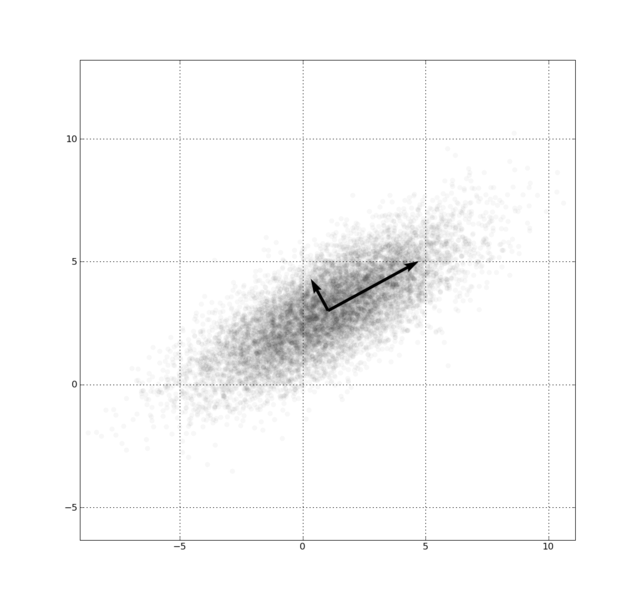
\includegraphics[width=0.8\textwidth]{2Dgaussian.png}
\label{fig:covariance image}
\end{figure}
\\As Figure \ref{fig:covariance image} shows, the covariance matrix can give extra information about the spatial distribution of a dataset.

This approach required more data to be compiled for each color. I created a separate small matlab code segment, which allowed me to select areas from an image, and save the RGB values of the contained pixels to a matrix. Then using another code segment I could use this dataset, to compile the $S$ covariance matrix and the $\mu_1$ mean which are needed for the calculation. I saved the pixel data along with the computed means and matrices to be able to load them from hard drive any time. With RGB the $R$ datapoint was a 3-dimensional vector, as well as $\mu_1$, and $S$ was a $3\times 3$ matrix.

Employing the Mahalanobis distance brought great results. After sampling enough pixels for each color using different images, the algorithm could correctly identify the bands as tight groups of large blobs -- after tinkering with the threshold value well.

To connect the blobs I used morphological closing: $n$ applications of morphological dilatation followed by $n$ applications of erosion using the same kernel. Here the value of $n$ and the kernel size was determined through trial-and-error as well, since these depend on the resolution of the image. To reduce remaining noise blobs I followed with the inverse morphological operation: opening -- first $n$ erosions, then $n$ dilatations.
\subsubsection{White-balance correction}
\label{subsec:white-balance matlab}
I noticed, that the lighting strength and color differed greatly even among resistors on the same picture, and this sometimes led to patchy color detection, since the pre-compiled color data was sometimes too "far away" from a color band which was a bit darker or brighter due to lighting.

We strived to solve this by introducing a some form of calibration. Since we started out with the assumption that the background is white, we figured that we could use that to get the RGB values which represent the white color in the actual lighting environment, and use that to calibrate the image.

My first idea was, that since I already have a mask of the resistors, I could use that to remove them from the background, and then calculate its average color. After I had the average $R, G \text{ and } B$ values, I calculated $V = max\{R,G,B\}$ and then found $r_1 \text{ and } r_2$ ratios with which the two non-maximum values need to be multiplied to be equal to $V$.

Then I went through each pixel of the masked resistor image, and multiplied the two appropriate channels with $r_1$ and $r_2$. This brought only slightly noticeable results, but was a slight improvement, and left it in the code nevertheless.

I will note here that I also introduced a pass of median-filtering on the masked resistor image before the Mahalanobis-distance calculation, since the images tended to have a bit of salt-and-pepper noise in lower light, and it also helped to remove tiny specks of bright highlight due to strong focused lighting.
\subsubsection{Actually detecting the bands}
Now that I had 10 binary masks with connected blobs representing bands, I had to go about processing this information into logical data, on which the value decoding process could be based.

My first step was to calculate the spatial centroids and areas of the blobs. Since I eventually had to measure the bands' distance, it immediately became clear, that this method is not robust enough. Even if the blobs were large and homogenous, sometimes they showed up on one top side of the resistor for one color, and the bottom side for another. If I just used these centroids, the resulting distance values wouldn't be representative of the actual distance of bands.

Thus I tried the following method. I used the mask of the resistor body to calculate the $\alpha$ orientation of the main axis of its bounding ellipse (the Image Processing Toolbox provides a very convenient function for this). Then using this angle I created the orientation vector $v=\lbrack1\quad tan(\alpha)\rbrack^T$. \label{eq:orientation} This is the orientation vector of the line $l$ which passes through the origo (in this case the bottom-left corner of the masked resistor image), and is parallel to the main axis of the bounding ellipse.

With $v$ I could create the matrix of orthogonal projection onto $l$:
\begin{equation}
\mathbf{P} = \frac{v \cdot v'}{v' \cdot v}
\label{eq:projection matrix}
\end{equation}
By mutiplying an arbitrary $p=\lbrack x\quad y\rbrack^T$ point from the left with $\mathbf{P}$ one can get its orthogonal projection onto $l$. This is what I did with all of the blob centroids, after this a significantly more reliable distance calculation is possible.

There were other issues first however, for example sometimes a smaller noise blob survives the morphological opening, and this had to be filtered out. I used logical filtering: first I found out the area of the largest connected blob in all of the color band masks. And in the following I disregarded any blobs, whose area was smaller than 35\% of the largest area.

Also, it was a common occurrence that a single band was represented by two large, separate blobs on the mask. I had to merge them somehow. The algorithm is that I after projecting all the blob centroids on the line $l$, I order them by ascending $x$ coordinate. Then I calculate the distances between neighbours, and find the largest one. After this I go through the list of the ordered band centroids, and check if the distance of two neighbours is less than an arbitrary percent of the largest distance.\footnote{In the current implementation it's 20\%} If this is the case, I check if they're of the same color, if so, I merge them: the new centroid will be the algebraic mean of the coordinates of the two centroids.

After these steps I had a list of band centroids along the $l$ line, and their respective colors. With this data it was rather straightforward to do the calculation of the resistor value using according to the guidelines laid out in section \ref{subsec:color codes} on page \pageref*{subsec:color codes}.
\subsubsection{Gold and silver bands}
\label{subsec:gold matlab}
The reader might have noticed that in the previous sections I have only discussed the detection of solid color bands. This is because the gold and silver bands pose an entirely different problem. I have worked only with gold bands, but it is safe to assume that silver bands are very similar in nature due to the additive metal particles in the paint.

This became clear as soon as I started experimenting with edge detection: while the other bands sometimes produced nicely visible edges, the gold bands never did. It is because they do not appear as a homogenous color, the highlight is usually very bright yellow, then as we go along the curve of the resistor body this becomes brownish, all the way to very dark at the edges. Because there are so many different colors involved, intensity-based gradient calculations don't detect an edge for gold bands.

The per-pixel color detection using the Mahalanobis distance also fails. If I compile pixel data from a whole gold band, the variance will be so large, that when I use the same threshold as I use for other colors, large sections of the resistor body, and some other color bands will also be registered as "gold".

Upon encountering this rather annoying problem, we tried using other colorspaces. I tried HSV, using Mahalaobis, the results were almost identical to RGB. Then I tried \textit{Lab} using only the \textit{a} and \textit{b} channels (here the covariance matrix is only $2\times 2$ size). The immediately apparent problem with this was the brown color had extremely similar \textit{a} and \textit{b} values tot the thin line of background often visible next to the resistor body due to the mask not being perfect, so the brown color mask was always very well populated even in the absence of a brown color band.

My next idea was to use more information in the Mahalanobis-distance calculation. I figured that since the color of the gold band changed along the curvature of the resistor body, I should incorporate this into the calculation somehow. I tried doing this, by calculating a pixel's distance from the center line of the resistor body.

To get the equation of the center line I used the $\alpha$ orientation (see section \ref{eq:orientation}), and the $C = \lbrack x_C\ y_C\rbrack $ centroid of the resistor body mask -- having an orientation and a point on the line I could write up an equation in the form of
\begin{equation}
A x+B y + C = 0
\end{equation}, where $A=tan(\alpha)$, $B=-1$ and $C=y_C-A x_C$. 
Then to calculate the $d$ distance of a $p=\lbrack x_0\  y_0\rbrack $ point from the center line I used:
\begin{equation}
d=\frac{\abs*{A x_0 + B y_0 + C} }{\sqrt{a^2+b^2}}
\label{eq:center distance}
\end{equation}
Having able to calculate this $d$ distance I created a new region-sampling program, which - additionally to the RGB values - also collected a given pixel's $d$. This way the $R$ in equation \ref{eq:Mahalanobis} became 4-dimensional, and $S$ became $4\times 4$. I also made sure to normalise the value of $d$, I use the length of the main axis of the bounding ellipse of the resistor body mask for this.

Having written this more complex code I was disappointed to find that the result was still entirely useless, too many areas were detected as gold.

After such trials I decided I have to abandon per-pixel detection for gold bands, I wanted to try a region-based method.

The first version of the algorithm was the following. I kept the extended, 4 element $R$ vector, but tried to sample multiple pixels. The sampling algorithm is like this: after the detection and processing of the solid band colors is done, and there is a possibility of a gold band existing (e.g. there are only 3 or 4 bands found), the sampling will begin at the centroid of the outermost color band, which is closest to the centroid of the resistor body (the "last" solid color band). Then the sampling continues along the center line of the resistor, towards closer end of the center line.

The center line is not smoothed, each center line point is calculated with taking either an integer $x$ or an integer $y$ coordinate, and calculating the other coordinate from that based on the already established equation of the center line. This can be problematic if, for example the $\alpha$ angle is near $90^{\circ}$, and we us integer $x$ coordinates to get the $y$ ones, our line will be very sparse. To counter this I switch between using $x$ and $y$ as basis for the other depending on $\alpha$. If $\alpha > 45^{\circ}$ I use integer $y$-s, otherwise $x$-es.

As the sampling advances through each center line point, it gathers pixels in a line which is perpendicular to the center line. This pixel collection starts at the center line point, extends in both directions along the perpendicular line, and stops when in one direction the next sampled pixel is pitch black - meaning that we reached the edge of the resistor mask. This produces an array of pixels for each point in the center line.

The sampled pixels are stored in a FIFO-like buffer. This buffer knows how large is the array of pixels belonging to a center line point, and when a new center line point is sampled, the pixels belonging to the least recently sampled center line point are removed. This means that the size of the buffer changes with each step.

If the buffer has enough elements after a sampling step (the threshold was set by trial-and-error), evaluation will take place. In this I calculate a covariance matrix from the pixels currently in the buffer, and then calculate the 2-norm of the difference of this matrix, and a precompiled gold covariance matrix. I also normalis this value by dividing with the mean of the precompiled gold covariance matrix. I save the values I get for each center line point (if there weren't enough pixels at that point, a maximum value is saved).

This produces a function, which scores each sampled center line point. If the score is low enough (threshold is arbitrary again), I deem that center line point to be a gold one. If there are enough consecutive center line points which are deemed gold, I detect a gold band at their centroid.

This rather complex and tedious method finally gave acceptable results. I changed the algorithm by removing the $d$ distance-from-center-line value, and just going with RGB values, since the highlight was not necessarily in the center of the body - the lighting may come from a different angle. This modification further improved the results, and on the test images detection of gold bands became possible.
\subsection{Testing and transitioning to Android}
After reaching this point I took more pictures with more varied resistor types. I found that the algorithm worked well for some images, but failed for others. My assumption was that this is due to the varying lighting conditions, and insufficient preprocessing steps to correct them.

At this time I changed the resistor body mask detection by creating an edge-image using Sobel operator along with the saturation channel thresholding. After morphological gap-closing I used the logical \emph{and} of the two images to create a mask to be passed to the ultimate erosion process. This helped to avoid scenarios, when differently lit spots of background were detected as resistors, but did nothing to improve the robustness of the color detection.

However with my consultant we decided that this prototype algorithm was a good enough starting point to start the Android implementation. I thought that the preprocessing steps will be more hardware and platform dependent, and it would be wise to only really start investing in their development in the Android environment.
\section{Android application}
\subsection{First steps}
As I have never worked with Android, nor Java -- which I knew Android development was most commonly based on -- I began with looking up information on the internet. I downloaded the Android Development Toolkit \cite{ADT link}, and started doing beginner tutorials offered on \linebreak[4] \href*{http://developer.android.com/training/index.html}, the official Android training website.

At first I used the device emulator of the SDK, but it was too slow to work with. Soon I received a Samsung Galaxy Tab 10.1 \cite{galaxy tab}.

In almost two weeks I have come to terms with the basic structure of an Android application, and then how to get the camera working, which was essential for my work.
In the next sections I will provide only limited explanation for basic android concepts like \verb!Activity! or other basic Android-related Java classes. Also I will not go into detail about the technicalities, since they are about the use of Android, OpenGL and OpenCV, for which ample documentation is readily available. Detailed description of the inner workings of the application can be found in the next chapter, here I just write a brief summary of the key development steps I went through.
\subsection{Setting up the camera}
I followed the camera tutorial on the training website to create a framework which can open the camera on application startup, an display a camera preview on the screen. I also decided that the application should be entirely in landscape orientation -- at least while I'm testing on a tablet.

First I used the standard Android solution for providing a camera preview: a \verb!SurfaceView!. An autofocus option is available in the Galaxy Tab I worked on, but it didn't seem to do anything by its own volition, so I added a button to force autofocus.

I added a gesture recogniser to the preview surface, so the detection process could start when the user taps the screen. I could also save the location of the user's tap. I made the tap also start a new \verb!Activity!, in which the detection process would take place.
\subsection{Starting out with OpenGL}
After this we I decided that in order to improve detection speed I should try using the graphics processor available in almost all newer Android devices - such as the tablet I was using.

I did some research, and found that the only currently available way to directly program the GPU on Android was through the use of OpenGL ES. So I did some tutorials to get a hang of the basics. The most difficult part was to understand how to create a working OpenGL environment in Android using Java. Once I learned that I experimented with basic vertex and fragment shaders.

I learned that almost all image processing tasks should be done in the fragment shader, which does operations on each displayed pixel. This meant that I had to set up OpenGL in a way that the image to be processed fills out the viewport entirely, and there is a one-to-one association between pixels of the image and the viewport.

After this I started to implement the algorithm developed in Matlab, mainly using OpenGL. I wrote fragment shaders for morphological dilatation and erosion, and also for RGB to grayscale and RGB to HSV color space conversion.

To apply multiple passes of these operations I had to bind a framebuffer, and re-bind textures after each pass. The shaders themselves executed very fast (usually clocking in under 5ms), but the switching of shaders and texture binding caused an overhead much larger than the time spent on useful computation.
\subsection{Introducing OpenCV}
At this time I received the suggestion that I should try OpenCV. I have already heard about this open-source library which contained a vast array of image-processing tools ready for use. I was also thinking about the issue of cropping images, and some other steps of the algorithm, which seemed to be very complicated or not really sensible on a GPU. And transferring data between the GPU and the CPU memory is a known bottleneck, so I was concerned.

OpenCV is readily available for the Android platform, so I integrated the libraries, and started experimenting. I immediately implemented a step, where right after taking the picture, the whole image is cropped to 1/16-th of its area, the center of the cropping being the location where the user tapped. This is a concession on one hand: the user has to tap on a resistor, but it is useful for selecting a single resistor, if there are multiple ones or some other clutter present -- while also reducing the amount of pixels which need to be processed. I did the cropping with the help of OpenCV methods.

The next step I added was to resize the image to a $240\times 180$ resolution for creating the masked resistor image. I did this to speed up the morphological operations, because on the original size image they usually took up to 100ms, but after the size reduction they were under 5ms. Another very important benefit of the resizing was that it standardised the image size, so I could fix the morphological kernel size, and the number of passes.

I continued using OpenCV methods to implement the next parts of the Matlab algorithm. I implemented the ultimate erosion, got the resistor body mask. Then I scaled it back to the size of the original, full-resolution image. I also did the calculation of the $\mathbf{P}$ projection matrix (see equation \ref{eq:projection matrix}).

The next step was the Mahalanobis calculation. I took new pictures with the tablet, and used them to compile new color data using my Matlab-program. As OpenCV has a built-in Mahalanobis distance method, I tried using that, calling it for each pixel. This was the cycle finished around 130ms for a single color. For all ten colors this would make the application unbearably slow, so I had to find an alternative.
\subsection{Mixing OpenCV and OpenGL}
I immediately thought of the GPU, since it is designed for per-pixel operations, and hardware-optimised for high speed floating-point multiplications. Calculating the Mahalanobis distance is a natural fit for its capabilities.

So after getting the masked resistor image with OpenCV methods, I passed it as a texture into OpenGL. In the fragment shader I can output 4 float values per pixel -- normally these are RGBA channels -- but I can use this to calculate the Mahalanobis distance for 4 colors per rendering pass. A single rendering pass with my Mahalanobis shader runs for less than 5ms, and only 3 passes are required. If we approximate the OpenCV solution for 10 colors to run for 10.3 seconds, this is a 600-fold improvement in speed.

This increase is somewhat offset by the tame it takes to read the resulting masks from the GPU memory and split them into ten separate \verb!Mat!-s, the standard image container class OpenCV uses. This is an inevitable, yet negligible compromise when using the graphics processor.

I continued to implement the remaining steps of the algorithm with OpenCV. I experimented with different kernel sizes for making the detected bands homogenous, but had varying success, depending on how big the resistor was on the original picture (in other words from how far the user took the picture).

At this point I realised it was necessary to standardise the size of the image passed into OpenGL as well. Since this image could have an arbitrary aspect ratio depending on the resistor's orientation on the picture, I couldn't just set fix new dimensions. Instead, I experimented a bit until I found a kernel size and morphological operator pass number that worked for a certain picture distance. Then I checked that usually how many pixels does the masked resistor image contain, when the morphological operators perform well in creating noiseless, homogenous bands. Then I implemented a step which scales the image to have a very similar number of pixels to this number while maintaining its aspect ratio.

After this steps in optimal cases I had nicely connected and separate masks for detected colors. I then added the logic to get the band centroids, project them, calculate their distances, and so on.

I made an addition to this part of the algorithm compared to the Matlab version: now if multiple color band centroids are very close together, and there are more than one colors represented, the algorithm merges them together until only one band of each color remains, then chooses the color which has the largest area. The inspiration for this came from the cases where the focus was not sharp enough, and for example blobs of brown were detected at the ends of otherwise fully red bands. This new addition reliably fixes these cases.

\subsection{White-balance correction -- Android version}
I did some testing with the program, and found that usually the results were good, but sometimes, when the lighting was drastically different from the one present in the images from which I compiled the color data, detection became unreliable.

In other words I reached the level with the Android project where I stopped development of the Matlab algorithm.

I had a small detour trying the Lab color space again. This meant that I converted the source images in Matlab to Lab and compiled new Lab data. I also had to adjust the Mahalanobis distance calculation for 2D (the \textit{a} and the \textit{b} channel). I immediately hit the same obstacle as in Matlab: remaining visible bits of the background were all registered as brown.

Then my consultant suggested the use of white-balance correction. I thought of the corresponding part of the Matlab algorithm (see section \ref{subsec:white-balance matlab}). I soon realised, that the idea was good, but I missed a key step in Matlab. I only scaled up the value of the two channels which were not the largest to the value of the largest one. This made the background chromatically white, but didn't help too much with the color detection, as it depends on pre-compiled RGB values, which intrinsically contain the intensity along with chromaticity.

Now, in the Android application I wanted to upscale each channel to a preset level. This way both the chromaticity and intensity would be standardised for the image. I had to decide when to do the correction exactly.

I quickly came to the decision, that this white balance correction should be implemented already in real-time in the camera preview, so that the user can visually verify its correctness -- and to give a better feeling by providing brighter colors.

I knew that the Android implementation of OpenCV had a special camera preview solution, in which the developer has access to each preview frame as a \verb!Mat! class, and is free to any kind of processing on it before displaying it. Thus I created an alternative camera preview, using the OpenCV solution.

The first thing I noticed, that the framerate was much noticeably much lower than the standard \verb!SurfaceView! solution (around 15 frames-per-second). Then I tried to implement a color correction step in each display frame. It is somewhat complicated to do it with OpenCV, first I have to split the input image into separate channels. Then, because by default the color depth is 8bit in OpenCV, I have to convert the channels to at least half precision floating point format. Following this I have to apply the color correction ratios for each channel, and then merge them together. Doing this resulted in the unusable frame rate of 5 FPS.

Then I found out that in Android there is a way to pass the preview frames into OpenGL. This seemed like the perfect solution, since the GPU can perform the color correction in a single operation. I created another alternative preview solution with the OpenGL-based \verb!GLSurfaceView! class. I then wrote a simple fragment shader which does the multiplication with the ratios.

Now I actually had to determine these ratios. I came up with the following solution. If the user long-taps the preview surface, the next preview frame will be captured for processing. From this frame I construct three histograms for the RGB channels. Then I select the brackets in each histogram, which have the largest value. The color $\gamma =\{ R_1, G_1, B_1\} $ I get this way will be deemed as the background white color. This histogram-based method is in effect selecting the modus of the color values. All this of course assumes that the user orients the camera to a mostly white (more than 50\% of it has to be white) surface (such as a white sheet of paper). I want $\gamma$ to be perfectly white, and a preset intensity color $\Gamma = \{R_0,G_0,B_0\}$.\footnote{In the current implementation $\Gamma$ is 80\% of the maximum intensity white color} Then I calculate the $r_1=R_0/R_1, r_2=G_0/G_1, r_3=B_0/G_1$ ratios with which each channel has to be multiplied in the whole image.

After the new $r_1,r_2,r_3$ values are determined, they are updated in the GPU program, and the preview goes on with the new white balance correction. Calculating the ratios takes a bit of a time (with the compiling of the histograms and so on), but it only has to be one in a given lighting environment, and is only a slight visual hiccup in the preview. The added benefit of this method is that after the white balance correction is set, resistors can be placed on any relatively homogenous background, it doesn't have to be white.

Of course the main goal with this white balance adjustment was to improve detection. To incorporate the correction, I added the multiplication with the ratios to the fragment shader which does the Mahalanobis distance calculations. I do this, because the picture taken by the camera doesn't pass through the OpenGL shader which processes the preview frames, and thus it is not white balance corrected. And the easiest and fastest way to introduce the correction to the algorithm during the step already assigned to the GPU.

To test the effectiveness of this method I had to create white balance adjusted images to compile color data from -- so I added an extra button, which takes a picture, performs the white balance correction with OpenCV on a background thread (so the camera preview can continue in the meantime), and then saves it to the flash memory of the device. Using this I complied color data for red and brown colors.
\subsection{Value calculation logic}
As the final step I implemented an abridged version of the value calculation logic of the Matlab algorithm. It works for 3 and 4 band resistors, where the last band before the band coding the tolerance value is farther away from the previous one than the first two bands are from each other. This way many resistors can be accurately detected, but we have no information about tolerance, since I did not implement gold or silver band detection yet.
\subsection{Final tests}
Using resistors with only red and brown bands I did a few tests in largely different lighting. The addition of white balance correction improved the robustness of the algorithm greatly. When there was sufficient lighting, but it was strongly colored, the correction helped to produce reliable results. In very low light situations though, this linear upscaling of color channels doesn't solve the problem, because the sensitvity of the red, blue and green sensors in the camera change non-linearly in low light. This effect is evident with red bands, whose detection becomes spotty in weak light.
\section{Tasks for the future}
The largest remaining problem is the implementation of gold and silver band detection. A good starting point can be the already relatively reliable algorithm for this in the Matlab prototype (see section \ref{subsec:gold matlab}).

It can be safely assumed however, that that algorithm will have to be seriously refined and modified to be adaptable to different lighting conditions. This is because in low light, the characteristic bright highlight of the gold band is missing, it is mostly just yellow. One proposal I have is that maybe the device's flash can be used to take another picture after the no-flash one in quick succession, and use the flash-ed image for detection of the gold and silver bands.

Another task is to compile a reliable database of all ten solid colors for detection, and test each one under different lighting conditions.

Moreover, the display of the result of the calculation is only acceptable for debug purposes now, a rehaul of the user interface is required. This also means that testing on different devices is needed, like phones with smaller screens. On these devices maybe a different (portrait-oriented) layout will be needed.

Also, there are myriads of possible little changes which may greatly increase the detection speed. The most important ones are pre-loading the contents and classes of the \verb!Activity! which does the detection, so that the whole OpenGL environment does not need to be set up each time a detection process is started. The process currently runs on the UI thread, which means no user interaction while it's running. This has to be changed, the process has to be moved to a background thread (of hight priority), and a progress bar should be implemented to reassure the user of the correct operation of the application.

Finally, a thorough testing phase is necessary to iron out any unexpected bugs, as is usual with any software project.
\chapter{Documentation of the software}
\section{Matlab programs}
\subsection{Main program}
The prototype algorithm is implemented in the \verb!.m! file called ``res\_proto.m''.
By reading through this file, one can get deeper understanding of the algorithm, but I still cannot honestly recommend it, since many things are very Matlab-specific. The idea behind each step is explained in the previous chapter. Otherwise the program is commented to facilitate comprehension. I will not add any comments about it here.
\subsection{Programs for color data compiling}
These programs are in the the file ``pixel\_data\_extractor.m''. A separate program can be run by placing the cursor on a line in that program -- so that the corresponding section between the \verb!\% \%! separators is highlighted -- and pressing \verb!ctrl + enter!.

The first program can be used to gather RGB channel pixel date from a picture. First the user has to load the picture using the\linebreak \verb!Iresc = imread("filename.extension");! command in the Matlab command line. Then, upon running the program, a window will come up with the loaded image, and the user can draw a region-of-interest by clicking with the mouse. To close the region one may right-click. Then, right click on it again, and select the ``create mask'' option.

Upon this, the pixel data will be collected into the \verb!pixeldata! matrix in the main Matlab workspace. Each pixel is represented by a row in it, and the columns are R, G and B (assuming the loaded image was RGB of course).

The next program is like the first one, except this one only produces a two-column \verb!pixeldata! -- it only samples the second and third channels of the image. This can be used with the Lab color space to get the \textit{a} and \textit{b} channels.

Next up is another variant of the pixel data collector program. Prior running this, the full ``res\_proto.m'' program needs to be run. In that program, the user can change which image is loaded by altering line 50 in the code. After that, there is no need to manually load an image. This variant creates a 4 column \verb!pixeldata!, where the 4th value is the $d$ (check around equation \ref{eq:center distance}).

The next program is essential for sampling multiple bands of the same color, or expanding an already existing pixel database. To show its usage let's take building a new brown color database from scratch as an example.

\begin{enumerate}
\item First we need to load a picture of a resistor with a brown band. Then, run the first program, select the brown band, and finish. After this, we have a \verb!pixeldata! variable in the workspace.
\item Now, we need to copy this into another one which will hold all brown pixels -- let's call it \verb!brown_pixeldata! -- by calling \linebreak[1] \verb!brown_pixeldata = pixeldata;! in the command line.
\item Then, load another image with a resistor), and run the first program again to sample its brown band. Or, if the currently loaded image has multiple brown bands, sample the remaining ones first.
\label{enum:repeat step}
\item Here comes the fourth program. In it, we need to set the right side of the first assignment to our current pixel data collection variable's name. It is \verb!brown_pixeldata! in our example. Save, and run the program. After this, the \verb!pixeldata! variable will be appended by the new pixels from our second sampling.
\item Now, call \verb!brown_pixeldata = pixeldata;! again.
\end{enumerate}
To continue adding new brown pixels, repeat from step \ref{enum:repeat step}.

The last program takes the pixel data specified in its first line, compiles the $S$ and $\mu $  (check around equation \ref{eq:Mahalanobis}) for the Android application, and exports them into a file, which can be read by the app. The user can set the output filename by changing the first argument of the \verb!dlmwrite! function.
\begin{center}
\begin{framed}
A current task in the project is to compile color data for all colors except brown and red. Program 1, 4 and 5 need to be used for this among the above.
\end{framed}
\end{center}


\begin{thebibliography}{99}
\bibitem{ADT link} Android SDK installer download:\newline \href*{http://developer.android.com/sdk/index.html}
\bibitem{galaxy tab} Galaxy Tab 10.1 specification:\newline \href*{http://www.samsung.com/global/microsite/galaxytab/10.1/spec.html}
\end{thebibliography}
\end{document}